% Universidade Federal de Itajuba
% Instituto de Matematica e Computacao
%
% Modelo LaTeX para escrita de Trabalho de Conclusao de Curso
% para os cursos de Ciencia da Computacao e Sistemas de Informacao, em formato de artigo.
%
% Desenvolvimento:
% - Luiz Olmes Carvalho - olmes@unifei.edu.br
% - Rafael de Magalhaes Dias Frinhani - frinhani@unifei.edu.br
%
% Arte da capa:
% - Elisa de Cassia Silva Rodrigues - elisa.rodrigues@unifei.edu.br
%
%   ALTERE ESTE ARQUIVO APENAS NOS LOCAIS INDICADOS NOS COMENTARIOS

% Passe, entre os colchetes, a sigla do curso: cco/sin (letras minusculas)
\documentclass[cco]{imc}
\usepackage{float}

% Definicao dos dados do autor do trabalho
% Edite o arquivo 'configuracao.tex'
% Arquivo de configuracao do documento
% Define os dados do autor e do trabalho

% Nome do autor, exceto o sobrenome
% Por exemplo, para Edgar Frank Codd, ficaria:
% \autorNomeA{Edgar Frank}
\autorNomeA{Kelly dos Reis} % Este eh o primeiro autor

% Sobrenome do autor
% Por exemplo, para Edgar Frank Codd, ficaria:
% \autorSobrenomeA{Codd}
\autorSobrenomeA{Leite}

% Nome do segundo autor (se houver), exceto o sobrenome
% Seguir o modelo anterior para o autor A
% Se nao houver segundo autor, deixe o comando abaixo vazio,
% isto eh, sem nada entre as chaves, inclusive espacos em branco: \autorNomeB{}
\autorNomeB{}

% Sobrenome do segundo autor
% Seguir o modelo anterior para o autor A
% Se nao houver segundo autor, deixe o comando abaixo vazio.
\autorSobrenomeB{}

% Contato do(s) autor(es): informar o email
\emailAutorA{kelly.l.reis@gmail.com}
\emailAutorB{}

% O titulo do trabalho
\titulo{Plataforma Web Integrada para Fórum Acadêmico e Voluntariado}

% Dados do orientador
% Nome do professor orientador, exceto sobrenome
% Por exemplo, para Luiz Olmes Carvalho, ficaria:
%\orientadorNome{Luiz Olmes}
\orientadorNome{Bruno Guazzelli}

% Sobrenome do orientador
% Por exemplo, para Luiz olmes Carvalho, ficaria:
% \orientadorSobrenome{Carvalho}
\orientadorSobrenome{Batista}

% Dados do coorientador
% Nome do professor coorientador, exceto sobrenome
% Por exemplo, para Rafael de Magalhaes Dias Frinhani, ficaria:
% \coorientadorNome{Rafael de Magalhaes Dias}
% Se o trabalho nao possui coorientador, deixe o comando abaixo vazio,
% isto eh, sem nada entre as chaves, inclusive espacos em branco: \coorientadorNome{}
\coorientadorNome{}

% Sobrenome do orientador
% Por exemplo, para Rafael de Magalhaes Dias Frinhani, ficaria:
% \coorientadorSobrenome{Frinhani}
\coorientadorSobrenome{}

% Definicao de textos: preencha adequadamente
% Opcoes: Orientador, Orientadora, Coorientador, Coorientadora
\txtOrientador{Orientador}
\txtCoorientador{Coorientador}

% Ano de publicacao do trabalho
\ano{2026}

% Mes da publicacao do trabalho
% Nao se trata do mes da defesa, mas sim do mes em que foi realizada a entrega da versao final.
\mes{Julho}

% Local: nao altere
\local{Itajubá}

% Palavras chave: incluidas no fim do abstact e na ficha catalografica.
% Minimo de 3 palavras e maximo de 5 palavras.
% Se nao possuir as quarta e quinta palavras, deixe o campo vazio, sem nada entre as chaves, inclusive espacos em branco. Ex: \palavrasChaveD{}
\palavraChaveA{Fórum Acadêmico}
\palavraChaveB{ONGs Voluntárias}
\palavraChaveC{Plataforma Web}
\palavraChaveD{Engajamento Comunitário}
\palavraChaveD{Integração Universitária}

% Nome dos membros da banca examinadora: maximo de 5 membros
% Se a banca possuir menos membros, deixe os comandos vazios,
% isto eh, sem nada entre as chaves, inclusive espacos em branco. Ex: \membroBanca5{}
\membroBancaA{} % Normalmente, o primeiro membro da banca eh o orientador
\membroBancaB{}
\membroBancaC{}
\membroBancaD{}
\membroBancaE{}

% Data da defesa: para fins de preenchimento da folha de aprovacao
% Coloque o mes por extenso, como no exemplo abaixo
\dataDefesa{}

% Apos a defesa, adicione o scan do PDF da folha de aprovacao assinada ao seu projeto.
% Use o comando abaixo para indicar o caminho do arquivo. Ex: \pdfAprovacao{./figs/folha.pdf}
\pdfAprovacao{} % Para a versao de defesa, deixe este comando vazio, sem nada entre as chaves

% Pacotes ja carregados:
% algorithm2e, amsmath, amssymb, amsthm, array
% babel, caption, xcolor, enumitem, eso-pic, float
% ifthen, fancybox, fancyhdr, fontenc, geometry, hyperref
% graphicx, hyphenat, lastpage, lipsum, listings
% longtable, lscape, multirow, natbib, pdfpages
% pxfonts, rotating, setspace, subfigure, textpos

% Se necessario, adicione pacotes aqui.
% Use o comando \usepackage{}
% \usepackage{nome-do-pacote}
\usepackage{float} % Nao altere este comando

% Inicio do documento
\begin{document} % Nao altere este comando

% Gera a capa, folha de rosto, ficha catalografica e folha de aprovacao: obrigatorios no texto.
\maketitle % Nao altere este comando

% Secoes do texto: para inserir novas secoes, seguir o mesmo modelo abaixo.
\section{Introdução}
\label{introducao}

A comunicação acadêmica nas universidades brasileiras acontece de forma fragmentada. Na Universidade Federal de Itajubá (UNIFEI), o SIGAA e o Moodle convivem e se sobrepõem: os dois guardam material de aula, os dois organizam a entrega de tarefas e ambos oferecem alguma forma de fórum. Ainda assim, quando surge uma dúvida sobre o conteúdo de uma disciplina, a conversa migra para o WhatsApp ou para o e-mail. O problema, portanto, não é ausência de recurso. É que o recurso existe e não é usado, e a discussão termina em um canal onde se mistura com outros assuntos e some do alcance de quem venha a ter a mesma dúvida no semestre seguinte. Sobre esse movimento, \cite{kent2013} relata que os estudantes preferem as redes sociais informais em vez dos fóruns oficiais dos sistemas de gestão de aprendizagem.

Vale examinar por que isso acontece. Os fóruns desses sistemas foram construídos como um item a mais dentro de uma plataforma que existe para outra coisa — matrícula, nota, documento —, e herdaram a lógica administrativa do resto. As discussões não se organizam por disciplina de um jeito que o aluno reconheça, o que faz com que o conhecimento produzido em um semestre não fique disponível para os próximos. Outras universidades apresentam comportamento parecido, como a de São Paulo (USP), a Universidade Federal de Minas Gerais (UFMG) e a Universidade Estadual do Paraná (UNESPAR), que usam o Moodle ou sistemas próprios com fórum previsto, mas pouco frequentado. Seguindo essa linha de raciocínio, a revisão sistemática feita por \cite{almatrafi2019} sobre fóruns em cursos online mostra que esses espaços, quando bem integrados às disciplinas, auxiliam no engajamento dos estudantes, e \cite{kumi2023} acrescenta a essa discussão que, ao usar a análise de redes, verificou as interações dentro de um fórum, revelando o papel que cada aluno ocupa na troca de respostas.

Há ainda um terceiro espaço que fica de fora de todos esses sistemas. O trabalho em grupo ocupa boa parte da carga de várias disciplinas e é combinado inteiramente por fora: a turma se divide por mensagem, discute a repartição de tarefas em conversa privada e entrega o resultado sem que nada desse percurso passe pela universidade. Quando o grupo trava, a dúvida raramente chega ao professor. Levá-la até ele significaria expor a conversa inteira, e nenhum grupo faz isso. \cite{scager2016} observa que a aprendizagem colaborativa depende de condições criadas de propósito, e não apenas da reunião de alunos em torno de uma tarefa. O que se perde aqui não é só o registro da discussão, mas a chance de quem ensina perceber onde a turma está emperrada enquanto ainda há tempo de intervir.

O voluntariado universitário sofre de um mal parecido, com contornos próprios. Projetos de extensão, ONGs e a atlética divulgam suas atividades sobretudo nas redes sociais, o que restringe o alcance das oportunidades a quem acompanha na hora da publicação. Muitos alunos descobrem a vaga tarde demais, repassada por terceiros, ou depois que a inscrição já fechou. A UNIFEI tem o módulo de Ações de Extensão dentro do SIGAA, mas ele foi pensado para o servidor da instituição, e não para o aluno: a tela de busca traz mais de quinze filtros institucionais, como Área do CNPq, Centro da Ação, Edital, Programa Estratégico e Dimensão Acadêmica, parâmetros que fazem sentido para uma pró-reitoria e pouco ajudam quem apenas procura uma vaga de monitoria ou um projeto que combine com o seu curso. A participação segue igualmente manual. O coordenador envia uma lista à pró-reitoria de extensão, os certificados de participação são emitidos um a um, e cabe ao próprio aluno solicitar o aproveitamento dessas horas como atividade complementar no seu histórico. Sobre esse ponto, \cite{lopesjr2023} relata que não basta a universidade ofertar os projetos, sendo necessário um esforço intencional da instituição para que os alunos de fato participem das atividades de voluntariado.

Diante desses problemas, este trabalho desenvolveu uma plataforma web que reúne, em um único ambiente, um fórum acadêmico organizado por disciplina, um módulo de trabalhos em grupo e um sistema de voluntariado com certificação automática. No fórum, cada disciplina ganha o seu próprio espaço, e a pessoa enxerga apenas aquelas em que tem vínculo — o que evita que a dúvida de um oitavo período apareça para quem está no primeiro. Alunos, monitores e professores entram com perfis distintos e podem criar tópicos, responder, votar, marcar a melhor resposta e sinalizar quando uma resposta não resolveu, além de moderar o conteúdo das disciplinas em que atuam. A busca reconhece dúvidas equivalentes escritas com palavras diferentes. Esse detalhe responde diretamente ao problema do conhecimento que se perde: uma pergunta sobre laço que executa uma vez a mais e outra sobre erro de \textit{off-by-one} descrevem exatamente a mesma coisa sem compartilhar um único termo.

O módulo de trabalhos em grupo nasceu da lacuna descrita antes. O professor propõe a atividade, anexa o material de apoio e decide como as equipes se formam, por escolha dos alunos ou por sorteio. Cada grupo recebe uma conversa privada em tempo real, na qual o professor não entra. Quando a equipe emperra, ela marca a mensagem exata da dúvida e a encaminha à monitoria, que recebe aquele trecho e a descrição do impasse — nada mais. A solução preserva os dois lados da tensão: o grupo mantém a privacidade que o faz permanecer na plataforma em vez de migrar para aplicativos externos, e quem ensina passa a enxergar onde a turma está travando. No módulo de voluntariado, as organizações cadastram suas oportunidades, os alunos se inscrevem online e, ao encerrar a atividade, recebem automaticamente o certificado de participação, documento que instrui o pedido de aproveitamento das horas como atividade complementar e que hoje depende da rotina manual descrita anteriormente. Cada certificado carrega um código de validação pública, o que permite a qualquer instância verificar a sua autenticidade sem depender da organização emissora. Sustentando tudo isso, um sistema de notificações em tempo real avisa quando surge uma resposta em um tópico, uma mensagem no grupo ou a confirmação de uma inscrição.

O objetivo geral foi projetar, desenvolver e avaliar essa plataforma como resposta aos problemas relatados, com foco na comunidade acadêmica da UNIFEI. O percurso passou pelo levantamento bibliográfico nos eixos de comunicação em ambientes educacionais, fóruns de discussão, aprendizagem colaborativa e voluntariado universitário; pela análise comparativa entre as quatro instituições citadas; pela definição dos requisitos; pela especificação da arquitetura; pela modelagem do banco de dados em terceira forma normal; e pela implementação, que hoje conta com vinte e seis tabelas, cobertura automatizada de testes e as telas de todos os perfis em funcionamento. A documentação completa dos requisitos funcionais e não funcionais, junto ao código-fonte, está disponível no repositório do projeto\footnote{Disponível em: \url{https://github.com/kellyr5/plataforma-unifei}}, escolha que mantém este texto concentrado nas decisões de projeto em vez de reproduzir listagens extensas.

A metodologia é a de uma pesquisa aplicada de natureza qualitativa, conduzida pelo desenvolvimento experimental do sistema em abordagem incremental, com funcionalidades entregues em ciclos curtos e validadas antes do início do conjunto seguinte. As tecnologias foram organizadas por camadas: React.js, TypeScript e TailwindCSS na apresentação; Python com Django, Django REST Framework e Django Channels na aplicação; PostgreSQL como banco relacional e Redis para o gerenciamento de tokens e a comunicação em tempo real. O escopo foi delimitado como um produto mínimo apaixonante, denominado MLP (\textit{Minimum Lovable Product}), que reúne as funcionalidades essenciais e o cuidado com a experiência do usuário desde a primeira versão. A escolha se justifica por uma razão prática: a plataforma disputa espaço com canais informais já consolidados entre os alunos, como o WhatsApp, o e-mail e o Discord, e uma ferramenta institucional que exija esforço de adaptação sem oferecer ganho evidente tende a ser abandonada nas primeiras semanas \citep{kniberg2016}.

O restante do artigo segue assim: a Seção 2 apresenta os conceitos e trabalhos que fundamentam a proposta, com a análise comparativa entre as universidades; a Seção 3 detalha a arquitetura, os requisitos, a modelagem do banco de dados e os diagramas que representam o funcionamento da plataforma; a Seção 4 reúne os resultados obtidos com a implementação; e a Seção 5 traz as conclusões e os trabalhos futuros.

\section{Referencial Teórico}
\label{referencial}

Esta seção reúne os conceitos e trabalhos que sustentam a proposta: a comunicação em ambientes educacionais, o papel dos fóruns na aprendizagem colaborativa, o voluntariado no contexto universitário e as tecnologias escolhidas para o desenvolvimento.

\subsection{Comunicação em Ambientes Educacionais}

As universidades brasileiras operam vários sistemas em paralelo. Uns cuidam de matrícula, nota e documento; outros, de material de aula e entrega de tarefa. Cada ferramenta cumpre a sua finalidade dentro de um escopo isolado, e nenhuma delas foi projetada para a conversa que acontece dentro de uma disciplina.

Com a expansão das plataformas digitais, a comunicação entre estudantes se dispersou por canais informais como o WhatsApp e o e-mail, que não oferecem separação por disciplina, busca por conteúdo nem registro do histórico das interações \citep{alves2023}. Dúvidas já respondidas e orientações dadas por monitores se perdem, sem que novos alunos consigam recuperá-las. \citet{kent2013} observa esse movimento no ensino superior: os estudantes migram para redes informais em vez de usar os fóruns embutidos nos sistemas de gestão de aprendizagem. O ciclo se repete a cada semestre, quando os grupos são recriados pelos próprios alunos e descartados ao fim do período, junto com tudo o que foi discutido neles.

Não se trata de um incômodo operacional. \citet{kuh2009} demonstra que a qualidade das interações entre o estudante e a instituição influencia tanto o desempenho quanto a permanência no curso, o que desloca a ausência de um canal estruturado do terreno da conveniência para o do aprendizado.

\subsection{Fóruns de Discussão e Aprendizagem Colaborativa}

As plataformas acadêmicas brasileiras oferecem fórum, mas quase ninguém o utiliza. Na UNIFEI, o SIGAA disponibiliza uma aba de fóruns dentro da Turma Virtual de cada disciplina: na disciplina analisada, nenhum fórum havia sido criado no semestre corrente, e o fórum geral do curso de Ciência da Computação, mostrado na Figura \ref{fig-forum-curso}, tem seus últimos tópicos datados de 2019, todos sobre assuntos administrativos. No Moodle da instituição, os fóruns existentes se limitam às abas de avisos criadas automaticamente pelo sistema.

\begin{figure}[!ht]
\centering
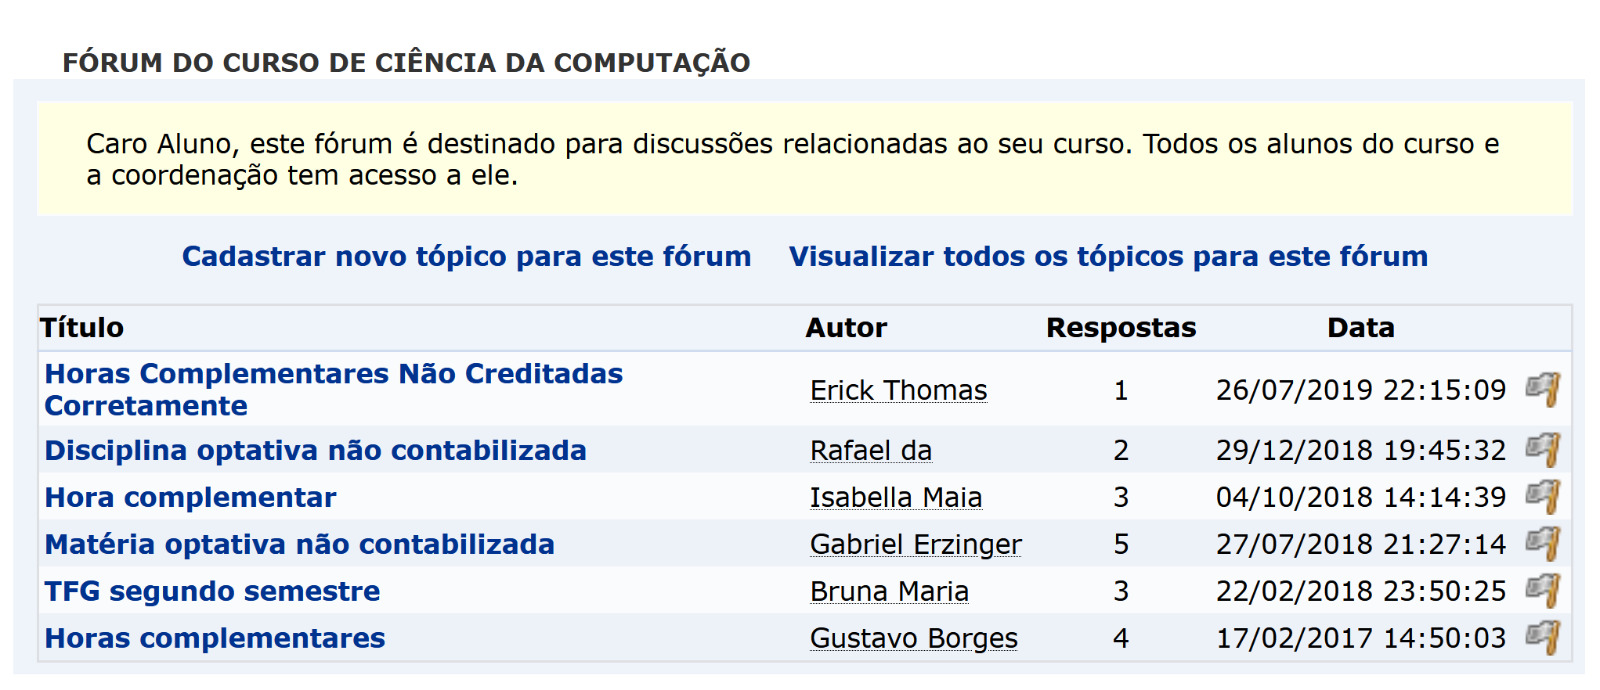
\includegraphics[width=\columnwidth]{figs/forum-sigaa-curso.png}
\caption{Fórum geral do curso de Ciência da Computação no SIGAA, com últimos tópicos de 2019.}
\label{fig-forum-curso}
\textit{\scriptsize Fonte: SIGAA UNIFEI (2026).}
\end{figure}

O padrão se repete nas demais instituições analisadas. A USP utiliza o e-Disciplinas, baseado no Moodle, sem ferramenta dedicada à discussão acadêmica; a UFMG combina o Moodle no UFMG Virtual com o sistema Siga, restrito a funcionalidades administrativas \citep{sigaufmg2019}; a UNESPAR adota o Moodle com o SIGES, voltado a solicitações burocráticas. Em todos os casos, o sistema acadêmico foi projetado para a gestão, e o ambiente de ensino, para a distribuição de conteúdo. A conversa ficou sem dono.

Parte da explicação está no desenho dessas ferramentas. \citet{bates2015} defende que o fórum não deve ser tratado como complemento do conteúdo, e sim como meio de construção do conhecimento, no qual os próprios alunos buscam recursos para fundamentar suas contribuições — o que exige recursos que sustentem a participação, e não apenas um espaço em branco onde publicar.

A base teórica dessa aposta vem da Teoria da Aprendizagem Social de \citet{bandura1977}, segundo a qual as pessoas aprendem comportamentos e atitudes observando umas às outras. Quando os alunos discutem, explicam e defendem ideias entre si, o esforço de organizar o raciocínio para apresentá-lo ao colega produz compreensão mais profunda do conteúdo. \citet{scager2016} acrescentam uma condição a isso: a aprendizagem colaborativa se torna efetiva quando existe interdependência positiva, ou seja, quando cada participante percebe que a sua contribuição é necessária ao resultado do grupo. Reunir alunos em torno de uma tarefa, por si só, não basta.

O Stack Overflow ilustra o que um ambiente projetado para essa finalidade consegue produzir: os usuários publicam dúvidas, outros respondem e a comunidade vota nas melhores respostas, que ganham destaque permanente \citep{vasilescu2014}. No contexto universitário, muitos alunos já improvisam algo semelhante no Discord, com servidores organizados por disciplina e canais para dúvidas e materiais. A demanda existe, portanto. O que falta é vínculo institucional, permanência do registro e diferenciação de papéis entre aluno, monitor e professor — sem a qual não há moderação possível nem forma de identificar a resposta confiável.

\subsection{Voluntariado Universitário}

O voluntariado contribui para a formação do estudante em duas frentes: desenvolve habilidades práticas, como liderança e trabalho em equipe, e constrói consciência social por meio do envolvimento com a comunidade. \citet{lopesjr2023} mostra, a partir de 259 respondentes, que a adesão cresce de maneira significativa quando a instituição se envolve ativamente — não basta disponibilizar os projetos.

Na UNIFEI, as ações de ONGs ligadas à extensão e as campanhas da atlética são divulgadas sobretudo no Instagram, sem plataforma que as centralize. O SIGAA possui um módulo de Ações de Extensão, apresentado na Figura \ref{fig-sigaa-extensao}, mas ele foi construído para a gestão administrativa: a tela de busca traz mais de quinze filtros institucionais, como Área do CNPq, Centro da Ação, Edital, Programa Estratégico, Dimensão Acadêmica e Unidade Proponente. São parâmetros úteis a uma pró-reitoria e inúteis a quem procura uma vaga compatível com o próprio curso. O módulo tampouco oferece inscrição direta ou comunicação com o coordenador do projeto.

\begin{figure}[!ht]
\centering
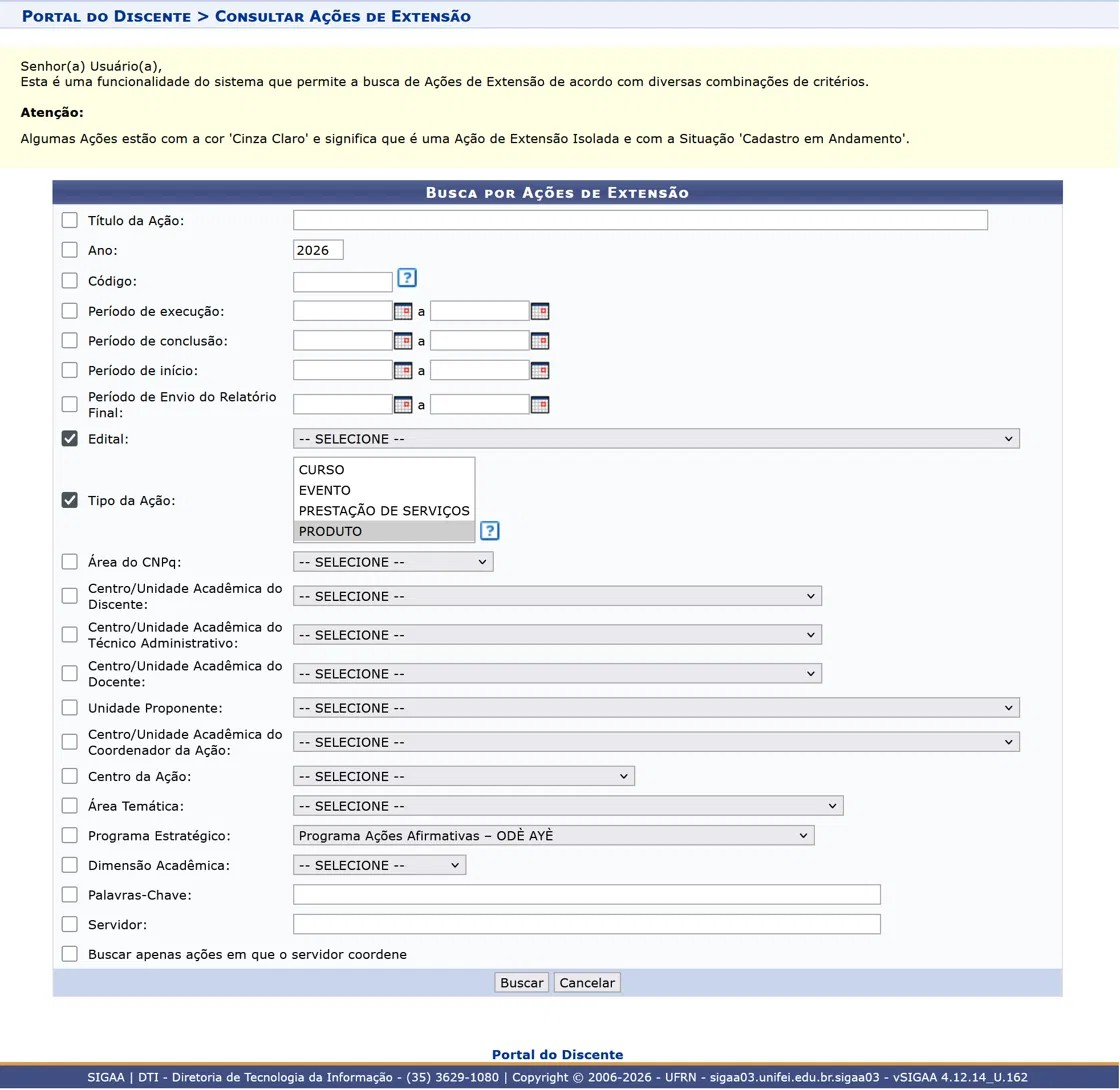
\includegraphics[width=\columnwidth]{figs/sigaa-extensao-busca.jpeg}
\caption{Tela de busca do módulo de Ações de Extensão do SIGAA da UNIFEI, com filtros voltados à gestão administrativa.}
\label{fig-sigaa-extensao}
\textit{\scriptsize Fonte: SIGAA UNIFEI (2026).}
\end{figure}

As outras instituições esbarram em limitações equivalentes. A UFMG mantém o SIEX, sistema de cadastro e gerenciamento de projetos de extensão, que permite consultar as atividades registradas mas não funciona como espaço no qual o aluno encontra oportunidades e se inscreve. Na UNESPAR, o registro das horas passa pelo SIGES em forma de solicitação burocrática, com o aluno selecionando manualmente a categoria do seu curso em um formulário, sem qualquer função de busca ou inscrição.

O custo dessa dispersão aparece depois que a atividade termina. Na UNIFEI, o coordenador solicita a emissão dos certificados à PROEX informando a matrícula de cada participante; em seguida, o próprio aluno pede o registro das horas no histórico, anexando o comprovante para que a coordenação do curso analise e aceite. São três etapas manuais para uma única participação, e o processo se repete de forma semelhante nas demais universidades analisadas. Como as atividades de extensão integram a grade curricular, a ausência de um fluxo que ligue inscrição, confirmação, certificado e registro de horas deixa de ser inconveniência administrativa e passa a ser obstáculo à própria integralização do curso.

\subsection{Análise Comparativa}

A Tabela \ref{tab-comparativo} sintetiza o levantamento, confrontando as funcionalidades oferecidas pelas plataformas das quatro instituições nos dois eixos examinados.

\begin{table}[!ht]
\centering
\caption{Comparativo entre as plataformas acadêmicas das universidades analisadas.}
\label{tab-comparativo}
\scriptsize
\begin{tabular}{|l|c|c|c|c|}
\hline
\textbf{Funcionalidade} & \textbf{UNIFEI} & \textbf{USP} & \textbf{UFMG} & \textbf{UNESPAR} \\
\hline
Sistema acadêmico & SIGAA & Júpiter & Siga & SIGES \\
\hline
Plataforma de ensino & Moodle & e-Disc. & Moodle & Moodle \\
\hline
Fórum disponível & Básico & Básico & Básico & Básico \\
\hline
Fórum efetivamente usado & Não & Não & Não & Não \\
\hline
Perfis por disciplina & Não & Não & Não & Não \\
\hline
Melhor resposta & Não & Não & Não & Não \\
\hline
Busca nos tópicos & Não & Não & Não & Não \\
\hline
Trabalho em grupo & Não & Não & Não & Não \\
\hline
Notificações em tempo real & Não & Não & Não & Não \\
\hline
Gestão de voluntariado & Ações Ext. & Não & SIEX & Não \\
\hline
Inscrição online & Não & Não & Não & Não \\
\hline
Registro de participação & Manual & Manual & Manual & Manual \\
\hline
Certificação integrada & Não & Não & Não & Não \\
\hline
\end{tabular}
\\ \vspace{5pt}
\textit{\scriptsize Fonte: Elaborado pela autora (2026).}
\end{table}

Nenhuma das instituições reúne, em um mesmo ambiente, um fórum com recursos que sustentem a participação e um sistema de voluntariado com inscrição, registro de horas e certificação automática. Os fóruns existem e não são usados; o voluntariado é gerido de forma descentralizada ou meramente burocrática; e o trabalho em grupo, que ocupa parte considerável da carga das disciplinas, não aparece em nenhuma das plataformas.

\subsection{Tecnologias Web}

Na camada de apresentação foram adotados o React.js, o TypeScript e o TailwindCSS. O React.js constrói interfaces a partir de componentes reutilizáveis, o que evita a repetição de um mesmo elemento em várias telas e facilita a manutenção conforme o projeto cresce \citep{react2024}. A escolha diante do Angular e do Vue.js considerou a curva de aprendizado, a maturidade do ecossistema e a presença da tecnologia no mercado brasileiro. O TypeScript acrescenta tipagem estática ao JavaScript, antecipando para o momento da escrita erros que só apareceriam em execução, e o TailwindCSS aplica estilo por classes utilitárias diretamente nos componentes, dispensando arquivos de estilo separados.

Na camada de aplicação, o Python com o framework Django oferece autenticação, painel administrativo, mapeamento objeto-relacional e proteções nativas contra ataques comuns, como CSRF (\textit{Cross-Site Request Forgery}) e injeção de SQL \citep{django2024}. O Django REST Framework organiza a construção da API por meio de serializadores e ViewSets, reduzindo código repetido nas operações de criação, leitura, atualização e remoção.

A comunicação em tempo real exigiu o protocolo WebSocket. No HTTP convencional, o cliente precisa consultar o servidor periodicamente para saber se algo mudou, prática conhecida como \textit{polling}; o WebSocket mantém uma conexão aberta e permite que a mensagem parta de qualquer um dos lados no instante em que o evento ocorre. A integração se dá pelo Django Channels \citep{channels2024}, que adiciona suporte ao protocolo ASGI (\textit{Asynchronous Server Gateway Interface}), com o Daphne como servidor de aplicação e o Redis como \textit{channel layer}, responsável por distribuir as mensagens entre as conexões.

O armazenamento ficou a cargo do PostgreSQL, banco relacional de código aberto que sustenta consultas complexas e oferece recursos como indexação textual e, por meio da extensão pgvector, busca por similaridade vetorial \citep{postgresql2024}. O Redis cumpre dois papéis: além do \textit{channel layer}, guarda os tokens de autenticação, dados de vida curta e escrita frequente que se beneficiam de um armazenamento em memória e que não precisam ocupar o banco relacional.

\section{Desenvolvimento}

Esta seção apresenta a solução proposta neste trabalho e detalha os elementos
técnicos que sustentam a sua concepção. Aqui são abordados os requisitos
funcionais e não funcionais que foram levantados, a arquitetura do sistema, a
modelagem do banco de dados em terceira forma normal e os diagramas que ajudam a
mostrar como a plataforma funciona, como ela é estruturada por dentro e como
fica a sua infraestrutura.

\subsection{Requisitos do Sistema}

Para que o desenvolvimento seguisse uma direção bem definida, foram levantados
os requisitos funcionais e não funcionais do sistema. Os requisitos funcionais
descrevem o que se espera que a plataforma faça do ponto de vista do usuário,
enquanto os não funcionais tratam de aspectos como segurança, desempenho,
disponibilidade e escalabilidade, que não aparecem direto para quem usa, mas
que sustentam o sistema por trás. A Tabela \ref{tab-requisitos} traz os
principais requisitos funcionais separados por módulo.

\begin{table}[!ht]
\centering
\caption{Principais requisitos funcionais da plataforma.}
\label{tab-requisitos}
\scriptsize
\begin{tabular}{|l|l|l|}
\hline
\textbf{Código} & \textbf{Módulo} & \textbf{Descrição} \\
\hline
RF-AUT-001 & Autenticação & Login via CPF e senha \\
\hline
RF-AUT-003 & Autenticação & Recuperação de senha por e-mail \\
\hline
RF-AUT-007 & Autenticação & Ativação de conta por código \\
\hline
RF-FOR-001 & Fórum & Criar tópico vinculado a disciplina \\
\hline
RF-FOR-003 & Fórum & Responder tópicos \\
\hline
RF-FOR-009 & Fórum & Votar em respostas \\
\hline
RF-FOR-010 & Fórum & Marcar melhor resposta \\
\hline
RF-FOR-013 & Fórum & Restringir publicação por decisão pedagógica \\
\hline
RF-FOR-015 & Fórum & Busca semântica e textual nos tópicos \\
\hline
RF-FOR-018 & Fórum & Analisar denúncia com justificativa ao autor \\
\hline
RF-COL-001 & Colaboração & Propor trabalho em grupo com material de apoio \\
\hline
RF-COL-004 & Colaboração & Formar grupos por escolha ou sorteio \\
\hline
RF-COL-007 & Colaboração & Conversa privada por grupo, em tempo real \\
\hline
RF-COL-011 & Colaboração & Encaminhar dúvida do grupo à monitoria \\
\hline
RF-VOL-001 & Voluntariado & Cadastrar oportunidade \\
\hline
RF-VOL-003 & Voluntariado & Inscrição em oportunidade \\
\hline
RF-VOL-007 & Voluntariado & Emissão de certificado em PDF \\
\hline
RF-PRF-002 & Perfil & Editar perfil com imagem e biografia \\
\hline
RF-PRF-006 & Perfil & Acompanhar o próprio percurso por disciplina \\
\hline
RF-NOT-001 & Notificações & Notificações em tempo real \\
\hline
\end{tabular}
\\ \vspace{4pt}
\textit{\scriptsize Fonte: Elaborado pela autora (2026).}
\end{table}

Cada requisito possui a sua descrição funcional e técnica, a indicação do ator
responsável por usá-lo e o nível de prioridade, parâmetros que ajudam a definir
a ordem em que as funcionalidades vão sendo implementadas ao longo do projeto.

Ao longo do desenvolvimento, dois conjuntos de requisitos foram revistos. O
sistema de reputação e o ranking semestral, previstos inicialmente para
incentivar a participação, foram removidos do escopo. A decisão partiu da
constatação de que a pontuação pública desloca o incentivo de ajudar para o de
pontuar, e de que esse deslocamento é mais visível em um fórum de disciplina,
no qual as mesmas pessoas convivem ao longo de todo o semestre, do que em uma
comunidade aberta e numerosa. O reconhecimento permaneceu apenas na marcação de
melhor resposta, que serve a quem consulta o tópico depois. Em contrapartida,
foi incorporado o módulo de colaboração, com trabalhos em grupo, conversa
privada por equipe e encaminhamento de dúvida à monitoria, respondendo a uma
lacuna identificada durante o levantamento: a discussão de trabalho em grupo
acontecia integralmente fora dos sistemas da universidade.

\subsection{Arquitetura do Sistema}

A arquitetura da plataforma foi pensada para separar as responsabilidades de
cada parte do sistema, como mostra a Figura \ref{fig-arquitetura}. O usuário
acessa a plataforma pelo navegador, que conversa com o frontend desenvolvido em
React.js com TypeScript e estilizado com o TailwindCSS. Esse frontend, por sua
vez, faz requisições HTTP à API REST do backend construído em Django com o
Django REST Framework, que é quem cuida da lógica de negócio, das validações e
das regras de acesso. O backend se conecta ao PostgreSQL para guardar os dados e
ao Redis para gerenciar os tokens JWT, os refresh tokens e as sessões que estão
ativas. Já para as funcionalidades que precisam de tempo real, como as
notificações e os chats, o navegador mantém uma conexão WebSocket direta com o
servidor de aplicação, gerenciada pelo Django Channels, o que permite enviar e
receber mensagens sem precisar ficar atualizando a página na mão.

A busca do fórum conta ainda com um componente opcional de recuperação
semântica, descrito na Subseção \ref{busca-semantica}, que utiliza a extensão
pgvector do PostgreSQL para armazenar representações vetoriais das publicações.

\begin{figure}[!ht]
\centering
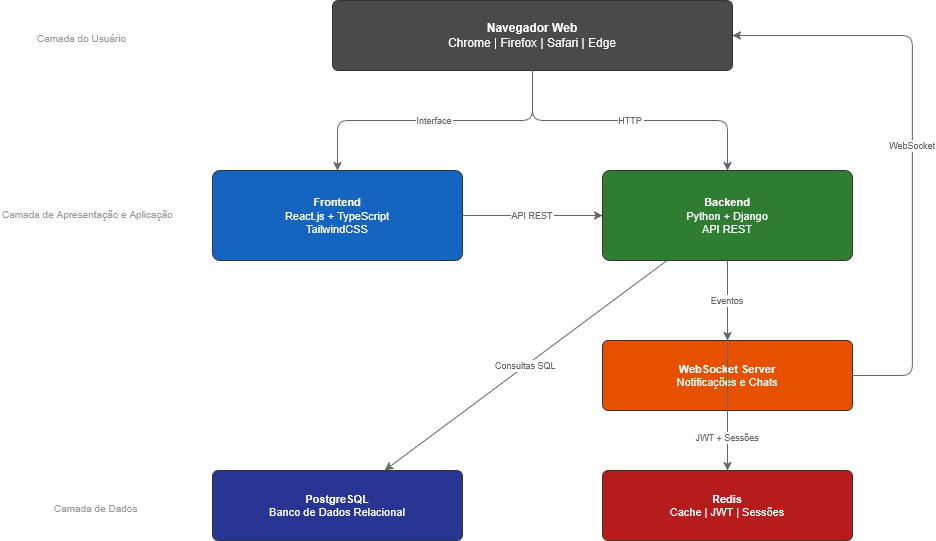
\includegraphics[width=\columnwidth]{figs/arquitetura.png}
\caption{Arquitetura do sistema proposto.}
\label{fig-arquitetura}
\textit{\scriptsize Fonte: Elaborado pela autora (2026).}
\end{figure}

Essa separação em camadas traz algumas vantagens para o sistema. Ela dá mais
modularidade, facilita a manutenção de cada parte de forma independente e ainda
permite que cada pedaço do sistema seja escalado conforme a demanda for
crescendo. Além disso, o fato de a camada de apresentação ficar separada da
camada de aplicação acaba abrindo caminho para uma evolução futura em direção a
aplicativos móveis nativos, já que a API REST construída pode ser consumida por
qualquer cliente compatível, e não só pelo frontend web.

\subsection{Modelagem do Banco de Dados}

A modelagem do banco de dados foi feita em terceira forma normal (3FN)
\citep{date2003}, o que ajuda a deixar as informações organizadas sem repetição
e com a integridade referencial preservada. O banco conta com 26 tabelas
espalhadas em seis módulos, como mostra a Tabela \ref{tab-banco}, agrupadas
de acordo com a funcionalidade que cada uma atende dentro do sistema.

\begin{table}[!ht]
\centering
\caption{Tabelas do banco de dados organizadas por módulo.}
\label{tab-banco}
\scriptsize
\begin{tabular}{|l|p{5.2cm}|}
\hline
\textbf{Módulo} & \textbf{Tabelas} \\
\hline
Autenticação & Usuario, CodigoAtivacao, RoleGlobal \\
\hline
Fórum & Curso, Disciplina, PermissaoDisciplina, Post, HistoricoEdicao, Voto, ReacaoPersiste, Arquivo, AlertaConteudo \\
\hline
Colaboração & Trabalho, ArquivoTrabalho, GrupoTrabalho, MembroGrupo, Conversa, ParticipanteConversa, MensagemChat, SolicitacaoAjuda \\
\hline
Voluntariado & Oportunidade, InscricaoVoluntariado, Certificado \\
\hline
Notificações e Auditoria & Notificacao, AuditLog \\
\hline
Busca & IndicePost \\
\hline
\end{tabular}
\\ \vspace{4pt}
\textit{\scriptsize Fonte: Elaborado pela autora (2026).}
\end{table}

A tabela Curso e os campos de período, carga horária, ementa, pré-requisitos e
co-requisitos em Disciplina permitem que a matriz curricular seja importada
diretamente do Projeto Pedagógico do Curso, em vez de cadastrada manualmente.
A oferta de cada semestre é derivada da paridade do período: disciplinas de
período ímpar são ofertadas no primeiro semestre e as de período par, no
segundo.

Vale registrar uma constatação da implementação. O PPC do curso de Ciência da
Computação declara o período de oferta de cada disciplina em dois pontos
distintos do documento, e eles divergem em quatro casos. A plataforma segue o
ementário, que organiza as disciplinas em grades por período e corresponde ao
desenho da oferta semestral efetivamente montada pela coordenação. A
divergência não seria percebida em uma leitura do documento, mas se torna
visível quando ele é traduzido em estrutura de dados, o que ilustra um efeito
secundário da informatização de normas acadêmicas: a implementação fiel expõe
inconsistências que o texto acomoda.

Durante a modelagem, foram tomadas algumas decisões pensando na segurança, na
auditabilidade e na manutenção do sistema. Todas as tabelas usam o UUID
(\textit{Universally Unique Identifier}) \citep{leach2005} como chave primária no
lugar dos identificadores sequenciais, uma escolha que dificulta a enumeração
dos recursos a partir das URLs e reduz o risco de expor dados internos sem
querer. As tabelas principais ainda contam com o campo \texttt{deleted\_at}, que
implementa a remoção lógica: em vez de apagar o registro, o sistema marca a data
em que ele deixou de valer, prática alinhada ao tratamento de dados orientados a
tempo descrito por \cite{snodgrass1999}. O conteúdo some da interface, mas
permanece recuperável em caso de exclusão indevida e disponível para auditoria.
Essa escolha convive com um limite: a Lei Geral de Proteção de Dados
\citep{brasil2018} assegura ao titular o direito à eliminação dos seus dados
pessoais, de modo que a remoção lógica não substitui a exclusão definitiva
quando ela for solicitada, e sim atende ao caso distinto da retirada de conteúdo
por moderação ou por engano do próprio autor.

O controle de acesso foi dividido em duas tabelas diferentes: a
PermissaoDisciplina, que cuida do papel do usuário dentro de cada disciplina
específica, permitindo que um mesmo aluno seja monitor em uma matéria e aluno em
outra, e a RoleGlobal, que fica com os papéis institucionais, como o de
administrador e o de organização, que não dependem de disciplina. Essa separação
coloca em prática o modelo de controle de acesso baseado em papéis (RBAC,
\textit{Role-Based Access Control}) \citep{sandhu1996} de um jeito mais
flexível, evitando que qualquer mudança no controle de acesso acabe mexendo na
tabela principal de usuários.

Sobre esse modelo, o sistema estabelece uma distinção que não se resolve apenas
com a hierarquia usual de papéis: a diferença entre supervisionar e participar.
A coordenação do curso responde por todas as disciplinas e precisa enxergá-las
por inteiro, mas não está matriculada em nenhuma turma e não leciona. Uma
implementação que trate o administrador como detentor de todas as permissões
faria com que a coordenação pudesse entrar em um grupo de trabalho, publicar
dúvida em uma disciplina que não cursa ou responder a um pedido de ajuda cujo
enunciado desconhece. A plataforma separa, portanto, dois predicados distintos:
um que autoriza a moderação de conteúdo, satisfeito também pelo administrador,
e outro que autoriza a condução da turma, que exige vínculo de professor ou
monitor com aquela disciplina específica. Organizar equipes, sortear grupos e
atender dúvidas de trabalho pressupõem conhecimento do enunciado, dos alunos e
do momento do conteúdo, e são atribuições de quem ministra a disciplina naquele
semestre.

A tabela AuditLog guarda todas as ações relevantes que acontecem no sistema,
registrando o endereço IP, o agente do navegador e o usuário responsável por
cada operação. Os registros dessa tabela não podem ser apagados em nenhuma
situação, o que garante a rastreabilidade que é necessária para fins de
segurança e de conformidade. Já os tokens de autenticação JWT (\textit{JSON Web
Token}) e os refresh tokens ficam guardados no Redis, e não no PostgreSQL, por
serem dados que mudam o tempo todo e que precisam de leitura e escrita rápidas,
algo em que um banco em memória acaba se saindo bem melhor que o banco
relacional.

\subsection{Diagrama Entidade-Relacionamento}

A Figura \ref{fig-er} mostra o diagrama entidade-relacionamento simplificado do
sistema, no qual as 26 tabelas aparecem agrupadas por módulo, com os seus
principais campos e os relacionamentos entre elas. Essa representação também foi
feita em terceira forma normal para evitar a repetição e garantir a integridade
dos dados que ficam guardados, mostrando de forma visual a mesma estrutura que
já foi descrita na Tabela \ref{tab-banco}.

\begin{figure}[H]
\centering
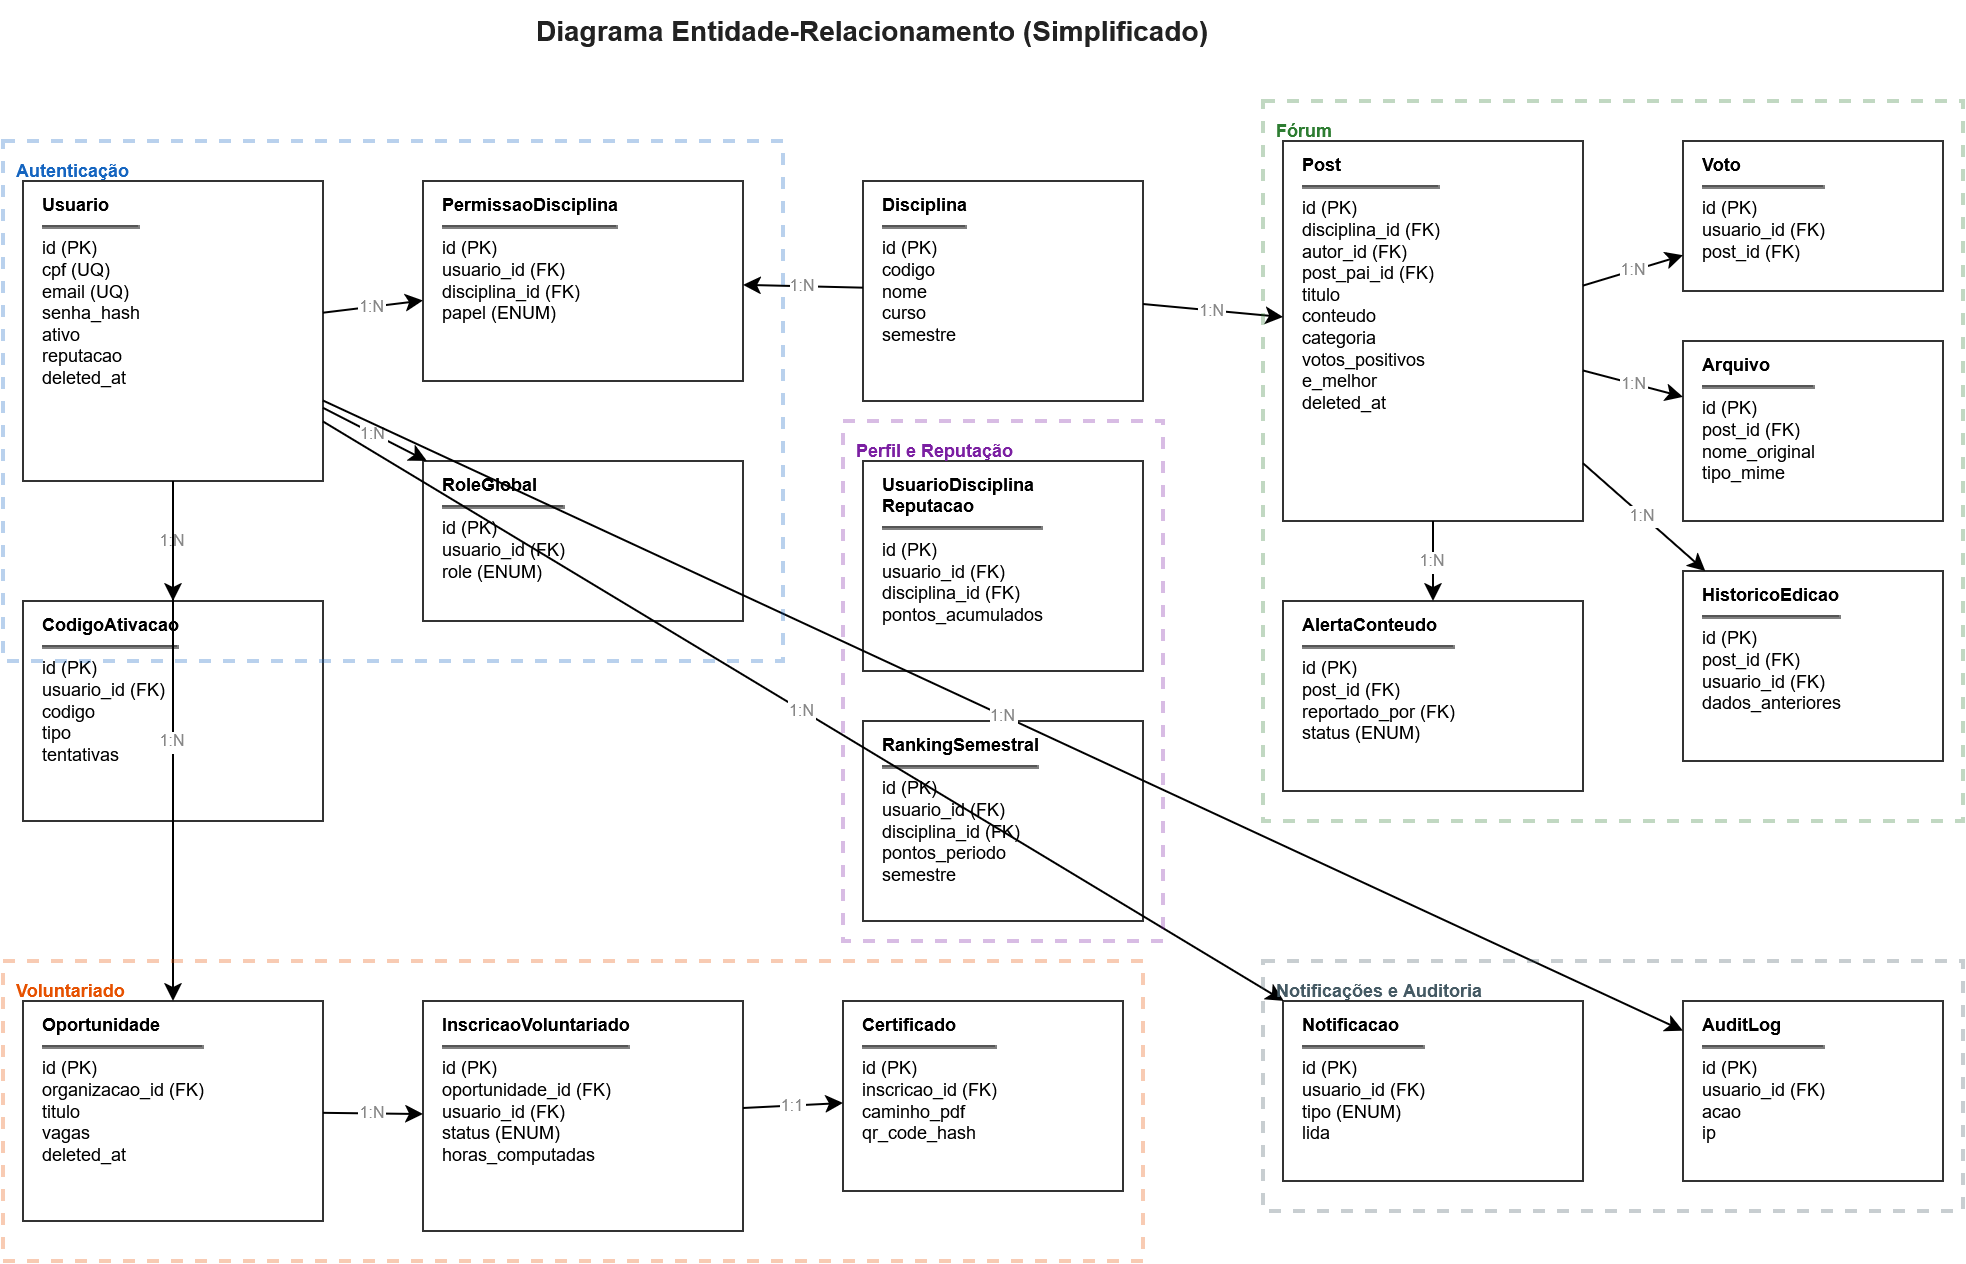
\includegraphics[width=0.50\textwidth]{figs/diagrama-er.png}
\caption{Diagrama entidade-relacionamento simplificado do sistema.}
\label{fig-er}
\textit{\scriptsize Fonte: Elaborado pela autora (2026).}
\end{figure}

\subsection{Recuperação Semântica de Publicações}
\label{busca-semantica}

Um fórum de disciplina acumula perguntas equivalentes formuladas com
vocabulários diferentes. As dúvidas ``por que meu laço executa uma vez a mais''
e ``erro de \textit{off-by-one} em vetor'' descrevem o mesmo problema e não
compartilham nenhum termo, de modo que a busca por palavra-chave jamais
relaciona uma à outra. O efeito prático é a republicação da mesma dúvida ao
longo dos semestres e a perda do conhecimento já registrado.

Para tratar esse caso, a plataforma incorpora um mecanismo de recuperação
semântica. Cada publicação é convertida em um vetor de 384 dimensões por um
modelo multilíngue de representação de sentenças \citep{reimers2019}, e esses
vetores são armazenados em uma tabela própria, indexada pela extensão pgvector
do PostgreSQL. A consulta do usuário passa pelo mesmo modelo, e a recuperação
ordena as publicações pela distância do cosseno em relação a ela, o que
aproxima textos por significado e não por coincidência de termos.

Três decisões de projeto orientaram essa implementação. A primeira é que os
vetores são gerados localmente, na própria infraestrutura, e não por serviço
externo: o conteúdo do fórum é material acadêmico de estudantes identificáveis,
e a transmissão desses textos a terceiros introduziria uma questão de
tratamento de dados pessoais desnecessária ao propósito do sistema. A segunda é
que o índice reside em tabela separada das publicações, de modo que a
substituição do modelo de representação implique uma reindexação isolada, e não
uma migração da estrutura do fórum. A terceira é que o recurso é opcional: na
ausência das bibliotecas correspondentes, a busca responde por correspondência
textual e nenhuma outra funcionalidade é afetada, o que evita que a
disponibilidade do fórum dependa de um componente acessório.

\subsection{Acessibilidade}

Por se tratar de sistema destinado a uma instituição federal de ensino, a
acessibilidade digital constitui obrigação legal, estabelecida pelo Decreto
n\textsuperscript{o} 5.296/2004 e pela Lei Brasileira de Inclusão
\citep{brasil2015}, e não recurso complementar. As diretrizes seguidas são as
da recomendação WCAG 2.1 \citep{w3c2018}, referência adotada pelo Modelo de
Acessibilidade em Governo Eletrônico brasileiro. A interface declara o idioma
português no elemento raiz do documento, condição para que leitores de tela
apliquem a pronúncia correta; mantém indicação visível de foco em todos os
elementos navegáveis por teclado; oferece atalho para o conteúdo principal como
primeiro elemento focalizável, evitando que a navegação percorra a barra lateral
a cada mudança de página; atribui rótulos acessíveis aos controles
representados apenas por ícone; e respeita a preferência do sistema operacional
por movimento reduzido. As combinações de cor foram verificadas quanto ao
contraste mínimo nos dois temas disponíveis.

\subsection{Casos de Uso}
\label{casos-de-uso}

\begin{figure}[!ht]
\centering
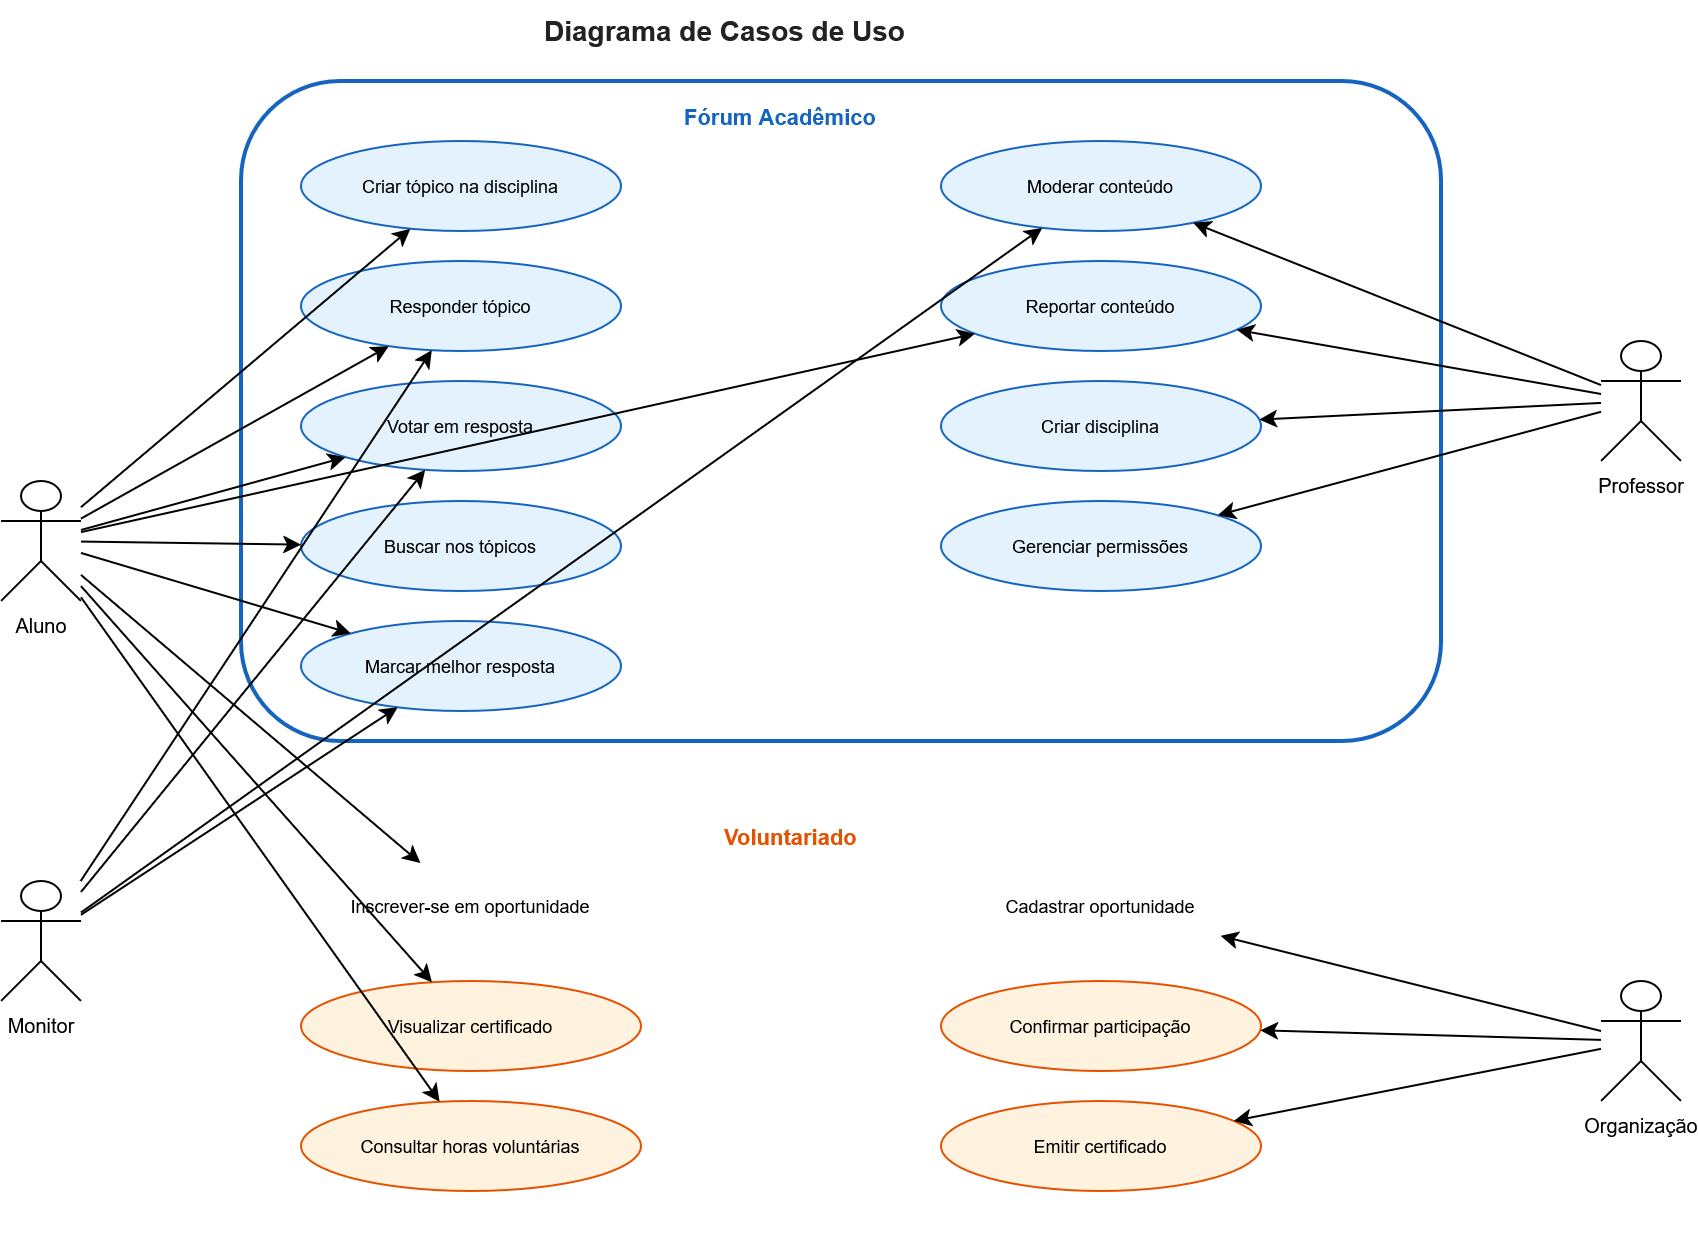
\includegraphics[width=\columnwidth]{figs/caso-de-uso.png}
\caption{Diagrama de casos de uso do sistema.}
\label{fig-casos-uso}
\textit{\scriptsize Fonte: Elaborado pela autora (2026).}
\end{figure}

A Figura \ref{fig-casos-uso} mostra o diagrama de casos de uso do sistema,
organizado em torno dos dois módulos centrais da plataforma: o fórum acadêmico e
o voluntariado. No módulo do fórum, o aluno pode criar tópicos, responder,
votar, fazer buscas e marcar a melhor resposta, enquanto o monitor e o professor
têm permissões a mais para moderar o conteúdo e cuidar das disciplinas. Já no
módulo de voluntariado, a organização cadastra as oportunidades e confirma a
participação dos alunos, enquanto o aluno se inscreve nas oportunidades, consulta
as horas que já tem registradas e visualiza os certificados que foram emitidos.

\subsection{Diagrama de Processos}

A Figura \ref{fig-processos} mostra o fluxo dos dois processos principais da
plataforma. No fórum, o aluno acessa a disciplina e faz uma busca nos tópicos
que já existem antes de criar um novo: caso ele encontre uma resposta que
resolva a sua dúvida, registra um voto e aquele conhecimento fica guardado para
as próximas consultas, e caso não encontre, cria um novo tópico que vai sendo
respondido por outros alunos ou monitores até que alguém marque a melhor
resposta e o tópico seja dado como resolvido. Já no voluntariado, a organização
cadastra a oportunidade, o aluno visualiza e se inscreve, participa da
atividade, a organização confirma a participação e o certificado é gerado
automaticamente, com as horas já registradas no perfil do aluno.

\begin{figure}[!ht]
\centering
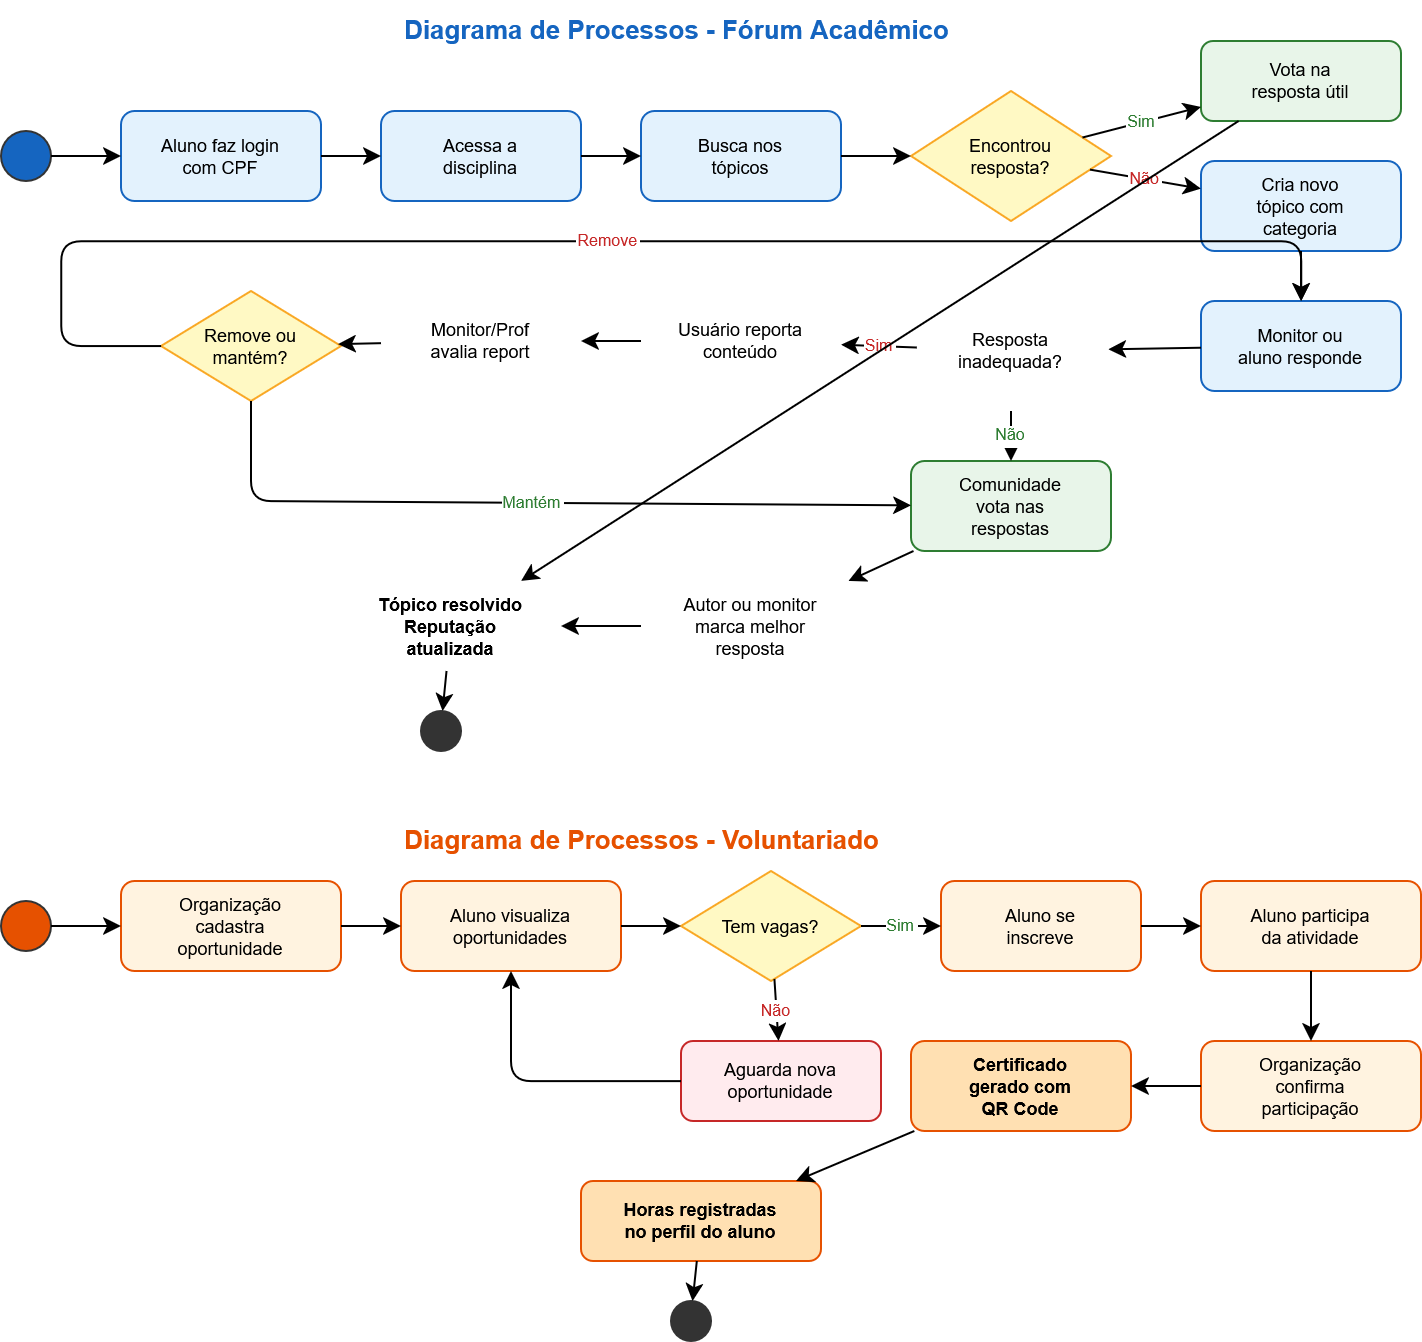
\includegraphics[width=0.5\textwidth]{figs/diagrama-processos.png}
\caption{Diagrama de processos do fórum acadêmico e do voluntariado.}
\label{fig-processos}
\textit{\scriptsize Fonte: Elaborado pela autora (2026).}
\end{figure}

\subsection{Diagrama de Implantação}

A Figura \ref{fig-implantacao} mostra como os componentes do sistema ficam
distribuídos em termos de infraestrutura. O usuário acessa a plataforma pelo
navegador, no qual o React.js roda localmente com a estilização do TailwindCSS.
As requisições passam por um servidor web Nginx, que entrega os arquivos
estáticos, como o HTML, o JavaScript e o CSS, e ainda funciona como proxy
reverso, mandando as chamadas da API REST para o servidor de aplicação, no qual
o Django roda junto com o Gunicorn (WSGI) para o tráfego HTTP comum, enquanto o
Daphne (ASGI) cuida das conexões WebSocket gerenciadas pelo Django Channels. O
Django se conecta ao PostgreSQL na porta 5432 para as operações com o banco e ao
Redis na porta 6379 para gerenciar os tokens JWT e as sessões ativas. As
credenciais de acesso ao banco e as outras configurações sensíveis ficam
guardadas em variáveis de ambiente, dentro de um arquivo \texttt{.env} que não
vai para o repositório do projeto, seguindo as boas práticas de segurança da
informação.
\begin{figure}[!ht]
\centering
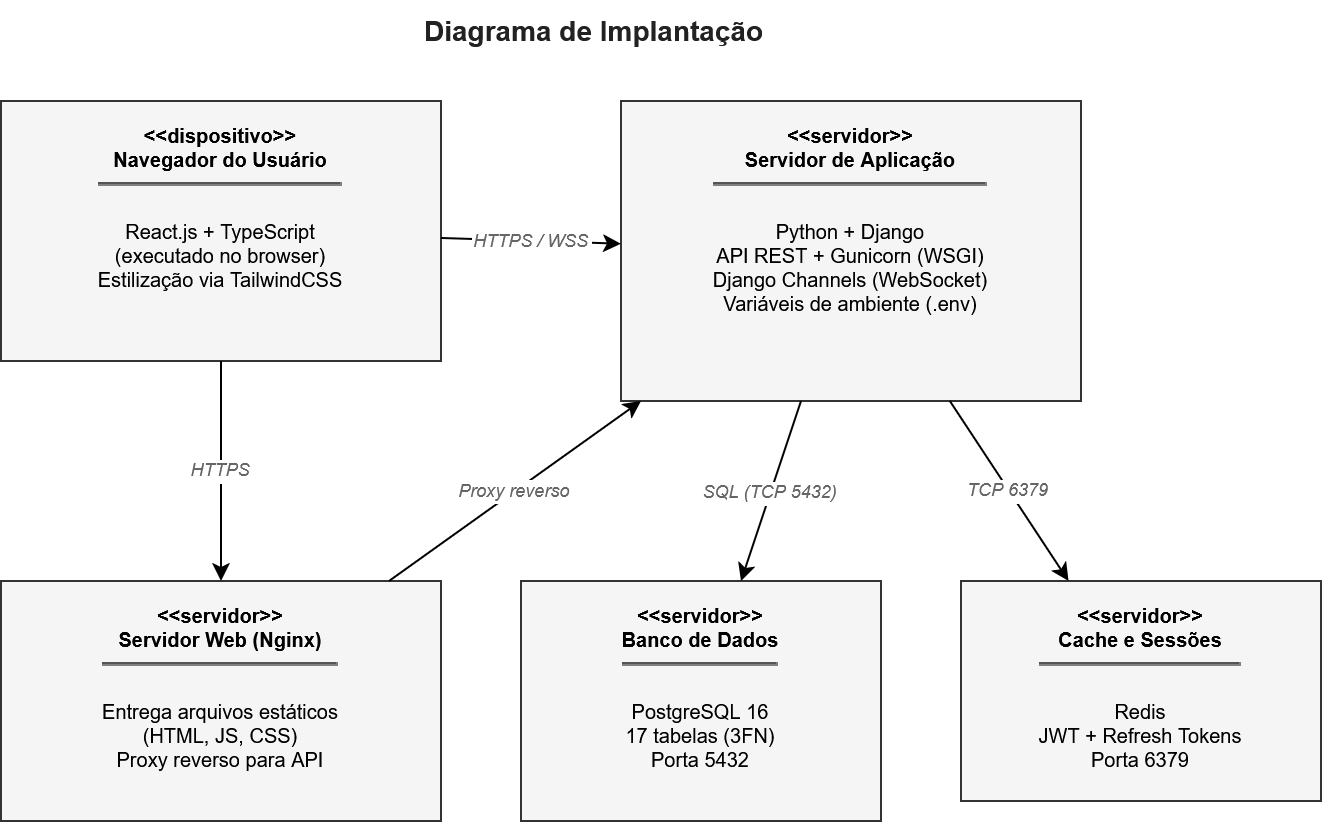
\includegraphics[width=0.50\textwidth]{figs/diagrama-implantacao.png}
\caption{Diagrama de implantação do sistema.}
\label{fig-implantacao}
\textit{\scriptsize Fonte: Elaborado pela autora (2026).}
\end{figure}

% As Consideracoes Parciais eram o fechamento do TCC-1, quando o sistema ainda
% era proposta. Com a implementacao concluida, o lugar delas passa a ser a
% Secao 4 (Resultados) e a Secao 5 (Conclusoes). O arquivo permanece na pasta
% como referencia enquanto as duas secoes nao estiverem escritas.
% \section{Considerações Parciais}

Este trabalho apresentou a proposta de uma plataforma web que junta um fórum
acadêmico organizado por disciplina e um sistema de voluntariado voltado para a
comunidade da UNIFEI. Foi feito o levantamento bibliográfico nos eixos de
comunicação em ambientes educacionais, fóruns de discussão, aprendizagem
colaborativa e voluntariado universitário, junto com a análise comparativa entre
as plataformas usadas pela UNIFEI, USP, UFMG e UNESPAR, que acabou deixando
claro algo que se repete em todas as instituições analisadas: a falta de uma
ferramenta que junte a discussão acadêmica estruturada com mecanismos de
engajamento e com uma gestão integrada do voluntariado.

A partir desse levantamento, foram documentados 53 requisitos funcionais e mais
de 30 requisitos não funcionais, foi feita a modelagem do banco de dados com 17
tabelas em terceira forma normal, foi definida a arquitetura do sistema com a
separação entre frontend, backend, banco de dados e cache, e foram construídos
os diagramas de entidade-relacionamento, casos de uso, processos e implantação.
O escopo do MLP foi delimitado dando prioridade às funcionalidades que entregam
valor e uma boa experiência ao usuário desde a primeira versão, contemplando o
login por CPF, a criação de tópicos ligados às disciplinas, a votação nas
respostas, a marcação de melhor resposta, a busca textual e, no módulo de
voluntariado, a inscrição nas oportunidades com a certificação integrada.

Para o TCC-2 estão previstas a implementação do protótipo funcional, usando o
React.js com TypeScript no frontend e o Django com o Django REST Framework e o
Django Channels no backend, e a realização de testes com usuários da UNIFEI
para validar se a plataforma de fato responde aos problemas que foram
levantados. Também está prevista a integração de um assistente inteligente ao
fórum, que vai reconhecer o que o aluno está procurando e direcionar a sua
dúvida para o lugar certo, seja o contato de um professor, uma informação da
UNIFEI, o material de uma matéria, um tópico parecido que já foi respondido
antes, a disciplina correta ou uma oportunidade de voluntariado, ajudando o
aluno a chegar mais rápido no que precisa sem se perder no caminho. Além disso,
está previsto o desenvolvimento das funcionalidades que ficaram planejadas para
as próximas versões, como as notificações em tempo real, o ranking semestral, a
moderação avançada e a integração com o SIGAA, deixando o sistema cada vez mais
perto de atender o que a comunidade acadêmica realmente precisa no dia a dia.
\section{Resultados}
\label{resultados}

Esta seção apresenta o que foi efetivamente construído, como o sistema se comporta em operação e quais verificações sustentam a afirmação de que ele funciona. A avaliação com usuários da comunidade acadêmica é tratada na Subseção \ref{avaliacao-usuarios}.

\subsection{A Plataforma em Operação}

A plataforma está implementada e em funcionamento, com os cinco perfis previstos ativos: estudante, monitor, professor, coordenação e organização parceira. A interface não é a mesma para todos. Cada perfil abre em uma página inicial construída a partir do que aquela pessoa precisa decidir, escolha que se mostrou mais produtiva do que apresentar um painel único com itens ocultos conforme a permissão.

O estudante entra em um painel que ordena as suas dúvidas colocando primeiro as que ainda não receberam resposta, acompanhadas dos trabalhos em grupo, das oportunidades de voluntariado abertas e do seu percurso por disciplina. O professor abre no que exige ação: quantas dúvidas aguardam resposta em cada uma das suas turmas, há quanto tempo aguardam e quantas denúncias esperam análise. A organização parceira não enxerga o fórum, porque não participa dele; sua tela reúne as oportunidades publicadas, as inscrições a avaliar e os certificados emitidos.

O painel da coordenação, apresentado na Figura \ref{fig-painel-coordenacao}, concentra a contribuição mais distante do que as plataformas analisadas oferecem hoje. Ele lista as disciplinas ofertadas no semestre corrente e, para cada uma, o número de dúvidas, quantas seguem sem resposta, a espera média até a primeira resposta, os estudantes ativos e as denúncias pendentes. A espera média é o indicador que dá sentido aos demais: poucas dúvidas com espera longa costumam indicar turma que desistiu de perguntar, e não turma sem dúvidas. As disciplinas sem professor ou sem monitoria atribuídos aparecem sinalizadas no topo, uma vez que a ausência de responsável explica boa parte da inatividade observada.

\begin{figure}[!ht]
\centering
\includegraphics[width=\columnwidth]{figs/painel-coordenacao.png}
\caption{Painel da coordenação, com os indicadores por disciplina do semestre corrente.}
\label{fig-painel-coordenacao}
\textit{\scriptsize Fonte: Elaborado pela autora (2026).}
\end{figure}

No fórum, cada pessoa enxerga apenas as disciplinas em que possui vínculo, e as dúvidas sem resposta aparecem separadas no topo, ordenadas da mais antiga para a mais recente. A busca opera em dois modos, conforme descrito na Subseção \ref{busca-semantica}, e informa qual deles respondeu — distinção que importa a quem procura, já que não encontrar nada por termo significa reformular a pergunta, enquanto não encontrar nada por significado significa que ninguém publicou algo semelhante.

O módulo de colaboração, mostrado na Figura \ref{fig-trabalhos}, apresenta os trabalhos propostos em cada disciplina com os grupos formados, as vagas restantes exibidas como posições em aberto e o material de apoio anexado pelo professor. A conversa de cada grupo funciona sobre WebSocket, com histórico recuperado por requisição HTTP na abertura, anexos, mensagens de voz e exclusão da própria mensagem dentro de três minutos após o envio.

\begin{figure}[!ht]
\centering
\includegraphics[width=\columnwidth]{figs/trabalhos-grupo.png}
\caption{Trabalhos em grupo de uma disciplina, com a composição das equipes e as vagas em aberto.}
\label{fig-trabalhos}
\textit{\scriptsize Fonte: Elaborado pela autora (2026).}
\end{figure}

No voluntariado, o percurso que hoje exige três etapas manuais foi reduzido a uma. A organização confirma a participação e o certificado é gerado em PDF, com código de validação pública que permite verificar a autenticidade do documento sem depender da organização emissora.

\subsection{Verificação por Testes Automatizados}

O comportamento do sistema é verificado por uma suíte de testes automatizados que cobre os módulos de autenticação, fórum, colaboração, voluntariado, notificações, auditoria e busca. Os testes exercitam tanto os caminhos esperados quanto as tentativas de uso indevido, e é nesta segunda categoria que reside a sua maior utilidade.

Regras de acesso falham em silêncio. Quando um recorte de permissão se rompe, nada na interface muda e ninguém percebe até que alguém veja o que não deveria. Por isso a suíte verifica explicitamente que um estudante não enxerga o fórum de disciplina em que não está matriculado, que o professor não acessa a conversa privada dos grupos da sua própria turma, que um integrante do grupo não visualiza pedido de ajuda alheio e que a coordenação, embora enxergue os trabalhos de todo o curso, não os organiza. Nesses casos, a resposta correta do sistema é negar a existência do recurso, e não recusar o acesso a ele: informar que algo existe mas está protegido já revela mais do que se deveria.

Três defeitos encontrados durante o desenvolvimento ilustram o tipo de erro que só aparece em uso real. O primeiro foi um botão de inscrição que existia, respondia ao clique e permanecia invisível, porque um valor de cor inválido invalidava toda a declaração de fundo e deixava texto branco sobre superfície branca — falha que não gera erro no console, não interrompe a compilação e não é detectada por teste de \textit{backend}. O segundo foi a exibição de vagas disponíveis com o rótulo de vagas preenchidas, o que fazia uma ação lotada informar zero ocupações ao lado de uma barra de progresso completa. O terceiro foi a coordenação recebendo a opção de ingressar em grupos de trabalho, consequência de tratar privilégio administrativo como se equivalesse a participação. Os dois primeiros foram corrigidos na interface; o terceiro exigiu a distinção entre supervisionar e participar descrita na Seção \ref{referencial} e passou a ser coberto por testes.

\subsection{Avaliação com Usuários}
\label{avaliacao-usuarios}

% ===========================================================================
% SUBSECAO PENDENTE — escrever apos a validacao com usuarios.
%
% Roteiro sugerido, para que o texto final tenha o que relatar:
%
%   - Perfil e numero de participantes (estudantes, monitores, professores)
%   - Tarefas executadas por cada participante. Ex.: publicar uma duvida;
%     localizar uma discussao anterior pela busca; entrar em um grupo de
%     trabalho; encaminhar uma duvida a monitoria; inscrever-se em uma
%     oportunidade de voluntariado
%   - Forma de coleta: observacao, questionario, escala SUS
%   - O que foi observado: tarefas concluidas sem auxilio, pontos de duvida,
%     tempo ate a conclusao
%   - Comentarios espontaneos e sugestoes recebidas
%   - Limitacoes: numero de participantes, ambiente controlado, ausencia de
%     uso ao longo de um semestre completo
%
% Esta subsecao responde ao verbo "avaliar" do objetivo geral. Sem ela, o
% objetivo fica parcialmente respondido.
% ===========================================================================

\textit{Esta subseção será redigida após a realização da validação com usuários da comunidade acadêmica da UNIFEI.}

\input{./elemtextuais/5-Conclusoes}

% Agradecimentos: elemento opcional
% Edite o arquivo 'elemtextuais/agradecimentos.tex'
% Deve ser uma secao sem numeracao (\section*{}), antes das referencias
% Para retirar essa secao, comente a linha a seguir.
\input{./elemtextuais/agradecimentos}

% Estilo da bilbliografia
\bibliographystyle{apalike2_ptBR} % Nao altere este comando

% Bibliografia no formato BibTeX:
% Edite o arquivo 'referencias.bib'
\bibliography{referencias}

% Apendices/Anexos: 
% Se muito necessarios, apendices/anexos devem ser inseridos como \section*{}
% Para inserir estes elementos, seguir o mesmo modelo abaixo.
%\input{nome-do-arquivo}

% Fim do documento
\end{document} % Nao altere este comando
